\chapter{A deep learning approach to estimate forward default intensities}

\section{Introduction}
\label{S:1}
The first default prediction models appeared forty years ago with the first generation model presented by \citet{altman}. This work led to the so-called Altman Z-score formula which uses accounting data to compute the default probability of a firm in the next two years. However, when used for financial firms, Altman's Z-score formula needs to be used with care  because, as I will discuss in this paper, financial firms have to be treated carefully due to their frequent use of off-balance sheet financing. Twenty years later, a second generation of reduced-form models used econometrical tools such as maximum likelihood, probit, and logit regressions. The major drawback of these models is that they do not provide multi-period forecasts. One innovative recent development is the use of doubly stochastic Poisson intensity model combined with multiple logit regression to account for multi-period default probability estimation. This model has been proposed by \citet{DSW} in \textit{Multi-period corporate default prediction with stochastic covariates}. The main contribution over prior work was to exploit the time-series dynamics of the explanatory covariates in order to estimate the likelihood of default over several future periods. Their model employs firm-specific and macroeconomic data to create a Markov state vector $X_t$ in order to compute independent firm default intensities $\lambda(t)$ and other types of exit intensities $\phi(t)$.
\citet{DSW} is the first model capable of multi-period default probability estimation using time dynamics of covariates $X_t$. Applications of \citet{DSW} works are various. We can find them in credit rating by credit rating agencies, banks who want to calculate the minimal amount of capital to be held and other researches analyzing the link between macroeconomic cycles and firm's default probabilities. Covariates used by \citet{DSW} are firm's distance to default, firm's trailing one-year stock return, three-month Treasury bill rate and trailing one-year return on S\&P500. Estimating their model on US-listed Industrial firms between 1980 and 2004, they find that distance to default and the current state of the economy have a significant impact on default hazard rates.

The two papers the closest to my paper are the work from \citet{DSW} and \citet{Duan2012}. The first model uses the doubly stochastic argument to derive multi-period default probabilities. To do so, it requires some strong assumptions (i.e Vectorial Autoregressive process) regarding the behavior of the time-series of covariates to generate future random values for the covariates. Obviously, if the process is misspecified, biases are introduced both in the forecasted covariates and in the future default probabilities. Five years later, \citet{Duan2012} shows that we can relax the VAR assumption with the use of forward intensities. This paper explains how we can reduce biases by projecting current event realizations on past data. For convenience, they specify the intensities as a linear function of state variables. I wish to extend the latter by removing the assumption of linear intensities and use an artificial neural network to estimate the intensities of the Poisson processes governing both default and other exits. 
Many papers on estimating default probabilities with machine learning techniques have already been written. For instance, \citet{barboza2017machine} test several machine learning models (support vector machines, bagging, boosting, and random forest) to predict bankruptcy one year prior to the event. They report a substantial improvement in prediction accuracy using these machine learning techniques especially when, in addition to the original Altman’s Z-score variables, six complementary financial indicators are included. To the best of my knowledge, such types of models do not rely on theoretical foundations and this is where the forward intensity model can contribute to the literature. It is able to provide multi-period predictions and is supported by a solid mathematical and econometrical background.

In \citet{DSW}, one of the main assumption is that the covariates governing both default and other exits intensities follow a high-dimensional vector auto-regressive (VAR) process. Using this type of process forces the model to greatly reduce either the number of firms in the sample or the number of state variables explaining firm attributes; if one does not restrict the number of firms or variables in the estimation, the dimension of the model will simply be too high and it will considerably increase computational time. A major step forward made in \citet{Duan2012} was to get rid off the VAR process in order to reduce computational time by using ``a new reduced-form approach based on a \textit{forward} intensity model''. These forward intensities produce a term structure of bankruptcy probabilities without using any sort of high-dimensional process. Using this method allows the model to incorporate a lot more state variables or individual firms in the sample. Moreover, \citet{Duan2012} state that their model may also improve robustness to misspecification because in a VAR model, estimation of future values are highly sensitive to any biases. On the other side, the forward intensity model approach is a ``direct projection of past data on current realizations'' which does not involve random estimation of future values. \\
Regarding covariates used, both \citet{Duan2012} and \citet{DSW} estimate their own Distance-to-Default (hereafter DtD). An important aspect to highlight is that distance to defaults specified in \citet{DSW} differ from those estimated in \citet{Duan2012} since the first one are estimated using the Variance Restriction method (see \textit{Measuring Distance-to-Default for Financial and Non-Financial Firms} \citep{Duan2012DTD}) and the second one using the transformed-data maximum likelihood estimation method to account for financial firms. The variance restriction method is a popular way to implement the \citet{Merton1974} model but fails to estimate properly the default point for financial firms. Following the KMV assumption (see \citet{KMV}), the default point in this method is specified as short term debt plus one half of long term debt and does not take into account other liabilities. However, it is well-known that financial firms such as banks specify a high portion of their debt as ``other liabilities". Hence, to include financial firms in the sample, the default point has to be adjusted to the sum of short term debt, one half of long term debt and a fraction $\delta$ of other liabilities. The method used by \citet{Duan2012} is using a maximum likelihood estimation in order to estimate the unknown fraction $\delta$. The Appendix provides additional methodological information on the DtD estimation using the variance restriction method and the maximum likelihood estimation. \\ 
To summarize, the forward intensity models require an assumption to link covariates to intensities. \citet{Duan2012} uses a linear assumption and a maximum likelihood to estimate those parameters. This paper contributes to previous literature by using neural networks to relax the linear assumption of forward intensities. Neural networks allow the estimation of highly non-linear functions without specifying the form of the relationships. The organization of the paper is as follows. Section 2 sets up the reduced-form model of default, develops the likelihood function used as loss function later on and describes the neural network approach. Section 3 discusses summary statistics of the dataset used. Section 4 presents the results. Section 5 concludes. Appendices at the end of the paper contains several proofs and more details on the Distance-to-Default estimation.


\section{Methodology}
\label{S:2}

\subsection{Default model}
\label{SS:2-1}

The model adds to the literature of reduced-form models of default for multiperiod corporate prediction using the doubly stochastic formulation as in \citet{DSW} (DSW henceforth) and \citet{Duan2012} (Duan henceforth). The default's time is modeled as the stopping time 
\begin{equation}
\tau_D = \inf\{t : N_t >0 , M_t = 0\},
\end{equation}
where $N_t$ and $M_t$ are the counting processes governing default and other exits respectively. Similarly, the stopping time for combined exits is denoted by
\begin{equation}
\tau_C = \inf\{t : N_t >0 \wedge M_t > 0\}.
\end{equation}

\noindent Naturally, we have the following :
\begin{equation*}
 \left.\begin{aligned}
        \text{if the firm exits due to default, } \tau_{Ci} = \tau_{Di},\\
        \text{if the firm does not exits due to default, } \tau_{Ci} < \tau_{Di}.
       \end{aligned}
 \right\}
 \qquad \text{$\Rightarrow \tau_{Ci} \leq \tau_{Di}$}
\end{equation*}


Let us denote by $Z_{it}$ the set of firm-specific variables at time t for the firm i and $Y_t$ the set of macroeconomic variables at time t. The first time of entry of the firm i is denoted  $t_i^0$. The econometrician's information set $\mathscr{F}_t$ at time t is thus
\begin{equation}
    \mathscr{F}_t = \{ Y_s : s \leq t \} \cup \mathscr{G}_{1t}  \cup \mathscr{G}_{2t} ... \cup \mathscr{G}_{Nt},
\end{equation}
where 
\begin{equation}
    \mathscr{G}_{it}  = \{  (1_{\tau_{C_i} < u} , 1_{\tau_{D_i} < u} , Z_{iu}) : t_i^0 \leq u \leq \min(\tau_D, \tau_C, t)  \}.
\end{equation}



\begin{figure}[H]
\label{lifespan}
\centering
    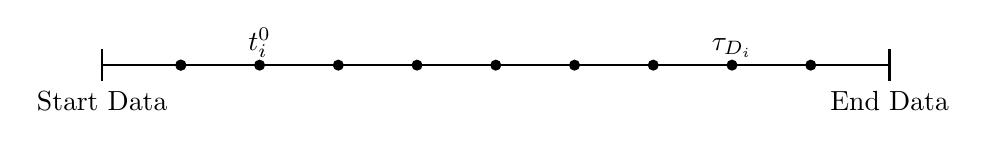
\begin{tikzpicture}[
dot/.style = {circle, fill=black,inner sep=0pt, minimum size=4pt},
every label/.append style = {inner sep=0pt, rotate around={0:(-0.5,1.5)}},
    thick      
                        ]
\draw ( 0,0.2) -- + (0,-0.4) node[below] {Start Data};
\draw (10,0.2) -- + (0,-0.4) node[below] {End Data};
%
\draw[thick] (0,0) -- node[below=2mm] {} + (10,0);
%
    \foreach \p in {0.1, 0.3, 0.4, 0.5, 0.6,0.7, 0.9}
{
    \node[dot] at (10*\p,0) {};
}
    \node[dot] at (10*0.1,0) {};
    \node[dot,label={$t_i^0$}] at (10*0.2,0) {};
    \node[dot,label={$\tau_{D_i}$}] at (10*0.8,0) {};

\end{tikzpicture}
\caption{Example of the lifespan of a firm. Each dot corresponds to a time period where the econometrician gathers firm-specific (if available) and macroeconomic variables. $t^0_i$ is the entry time of the firm i and $\tau_{D_i}$ denotes the default time of the firm i.}
\label{fig:lifespan}
\end{figure}

In Figure \ref{fig:lifespan}, each dot corresponds to a period. At each period, the econometrician gathers firm-specific variables (DTD, Cash/TA, NI/TA, ...) and macroeconomic variables (S\&P500 return, treasury rate). For a particular point in time t, the econometrician knows the whole time-serie of macroeconomic variables until t irrespective of $t_i^0$, and the time-series of firm-specific variables from $t_i^0$ to $\tau_{D_i}$ if $t_i^0 \leq t$ and $t \leq \tau_{D_i}$.
Following Proposition 1 in \citet{DSW}, the conditional probability of default within $s$ years can be computed as 
\begin{equation} \label{eq:3.6}
\mathbb{P}[ \tau_D <t+s |\mathscr{F}_t] = E_t \left[ \int_t^{t+s}  e^{-\int_t^z (\lambda(u)+\phi(u)) du} \cdot \lambda(z) dz \right].
\end{equation}
The probability of default is a function of intensities $\lambda$ (default) and $\phi$ (other exits). However, these intensities are unknown and unobservable. In DSW model, the state variables governing Poisson intensities are assumed to follow a specific vector autoregressive (VAR) process. This assumption is relaxed in Duan's paper by using forward intensity rates. Instead of modeling $\lambda_{it}$ and $\phi_{it}$ as some function of state variables available at time t, \citet{Duan2012} propose to deal with $f_{it}(\tau)$ and $g_{it}(\tau)$ directly as functions of state variables available at time t and the forward starting time of interest $\tau$. The analogy to interest rates would be that $\lambda_t$ is the short rate and $f_t(u)$ is the forward rate for horizon $u$. \citet{Duan2012} propose a model to predict corporate defaults at multiple horizons by estimating these forward intensities via maximum likelihood. To do so, they use a linear assumption in the relationship between the variables and the forward intensities (i.e $f_{it}(\tau) = \exp(\alpha_0(\tau) + \alpha_1(\tau) x_{it,1} + \alpha_2(\tau) x_{it,2} + ... + \alpha_k(\tau) x_{it,k}$). However, it is highly likely that default intensities depend on those covariates in a non-linear way. I propose to use an artificial neural network (ANN) to find the set of weights governing the process $f_{it}$ and $g_{it}$. I show that I am able to capture potential non-linear relationships between the state variables and the forward intensities which significantly improves forecasts.


\subsubsection{Forward intensities}
\label{SSS:2-1-1}

Since we do not have the exact knowledge of $\lambda$ and $\phi$, \citet{Duan2012} propose to use forward intensity rates. However, we need to translate the default probability given in equation \ref{eq:3.6} (which depends on spot intensities) into a formula that depends on forward intensities. To do so, we first compute the probability of surviving as a function of forward combined intensity, which will be later used to compute the probability of default as a function of both combined and default forward intensities. Let us denote by $F_{it}(\tau)$ the conditional distribution function of the combined (default and other exits) exit time evaluated at $t+\tau$. Hence, 1-$F_{it}(\tau)$ is the probability of surviving in the interval $[t, t+\tau ]$. Therefore, we have :
\begin{equation}
1-F_{it}(\tau) = \mathbb{E}[e^{-\int_t^{t+\tau} (\lambda(s)+\phi(s)) ds}].
\end{equation}
Then, let us introduce the quantity $\psi_{it}(\tau)$ to be :
\begin{equation} \label{eq:3.8}
\psi_{it}(\tau) \equiv -\frac{\ln(1-F_{it}(\tau))}{\tau} \equiv -\frac{\ln(\mathbb{E}[e^{-\int_t^{t+\tau} (\lambda(s)+\phi(s)) ds}])}{\tau}.
\end{equation}
Reverting equation \ref{eq:3.8} gives :
\begin{equation}\label{eq:psi}
e^{-\psi_{it}(\tau)\cdot\tau} = 1-F_{it}(\tau).
\end{equation}
Where $e^{-\psi_{it}(\tau)\cdot\tau}$ is again the survival probability. We now need to compute $\psi_{it}(\tau)\cdot\tau$. At this point, \citet{Duan2012} makes the assumption that $\psi_{it}$ is differentiable and defines the forward combined exit intensity as 
\begin{equation} \label{eq:3.10}
g_{it}(\tau) \equiv \frac{F_{it}'}{1-F_{it}}.
\end{equation}
Equation \ref{eq:3.10} comes from the definition of a hazard rate function. Referring  P.87 of \citet{book}, the definition of a hazard rate function is the following:
%\newtheorem*{mydef}{Definition}
\begin{definition}[Hazard rate]
Let denote by $\tau$ a stopping time and $F(T) \equiv \mathbb{P}[\tau \leq T]$ its distribution function. Assume that $F(T) < 1 \forall T$, and that F(T) has a density f(T). The hazard rate function h of $\tau$ is :
\begin{equation*}
h(T) \equiv \frac{f(T)}{1-F(T)}.
\end{equation*}
\end{definition}
A hazard rate is the local arrival probability of a stopping time per time interval. Please note that under suitable regularity conditions, intensities and hazard rates are closely similar. In particular, in our doubly-stochastic framework, hazard rates and intensities are equivalent. This is why in \citet{Duan2012}, we have $\lambda(t) = h(t)$ and the distinction between hazard rates and intensity is often not made. \\

\noindent The relation between $g_{it}(\tau)$ and $\psi_{it}(\tau)$  is given by :
\begin{align} \label{gphi}
    g_{it}(\tau) &= \frac{F_{it}'(\tau)}{1-F_{it}(\tau)} \nonumber \\
    &= \psi_{it}(\tau) + \psi_{it}'(\tau)\tau.
\end{align}

\noindent Then, we can compute the quantity $\psi_{it}(\tau) \tau$ that we were looking for as :
\begin{equation}
    \psi_{it}(\tau) \tau = \int_0^{\tau}g_{it}(s) ds.
\end{equation}

\noindent For an interested reader, proofs of the above formulations can be found in the Appendix. Hence, the probability of surviving over [t,t+$\tau$] is given by
\begin{equation} \label{survprob}
    \mathbb{P}[\tau_c > t+\tau |\mathbb{F}_t] = \exp(-\int_0^\tau g_{it}(s) ds).
\end{equation}

The forward default intensity for horizon $\tau$ is defined as the limit for a small time step of the probability of defaulting in this small time step given that the firm has survived. The probability is Bayesian and the forward default intensity denoted $f_{it}(\tau)$ is the following :
\begin{equation}
f_{it}(\tau) \equiv \dfrac{\lim_{\Delta t\to 0} \dfrac{\mathbb{P}[t + \tau < \tau_{Di}=\tau_{Ci} \leq t+ \tau + \Delta t]}{\Delta t}}{e^{-\psi_{it}(\tau)\cdot\tau}}.
\end{equation}
Hence, the probability of defaulting between t and t+$\tau$ is given by :
\begin{equation}\label{probdef}
\int_0^{\tau} e^{-\psi_{it}(s)s} f_{it}(s)ds = \int_0^{\tau} e^{-\int_0^s g_{it}(u) du} f_{it}(s)ds.
\end{equation}


\subsubsection{Likelihood function}
\label{SSS:2-1-2}

In this setup, the likelihood function depends on three types of probabilities (default, other exit and surviving) which themselves depend on the types of intensities (default and other exits). The negative log-likelihood function has to be adjusted to the neural network framework and can be used as objective function to be minimized as long as we feed mini-batches and not single data points (``online learning''). Mini-batch feeding is a common practice in machine learning papers and consists of splitting the available data in batches of fixed size. Then, each backward pass takes one batch to perform one gradient decent step.  \\

To allow further comparison with \citet{Duan2012},  I employ the same discretization of time: $t = 0, 1, 2,...$ and $\tau = 0, 1, 2,...$ are time sequences of one month increment. Similarly, $f_{it}(\tau)$ and $g_{it}(\tau)$ are forward intensities computed at time t for the period [t+$\tau$, t+$\tau$+1]. The use of the $\tau$ index is to account for multiperiod prediction. When $\tau = 0$, the forward intensity model is computing spot intensities. When we set $\tau = 1$, the forward intensity model produces estimates one step ahead, and so on so forth. I denote $X_{it} = (x_{it,1}, x_{it,2} ,...)$ the set of firm-specific and macroeconomic variables explaining both default and combined exit intensities. As specified in \citet{Duan2012} $f_{it}(\tau)$ and $g_{it}(\tau)$ are functions of $X_{it}$ and can be specified as any form of function as long as they satisfy the following constraints. Since combined exit intensity has to be greater or equal than default intensity, we need to make sure that the forms specified for $f_{it}(\tau)$ and $g_{it}(\tau)$ satisfy the following conditions : $f_{it}(\tau) \leq g_{it}(\tau)$, $f_{it}(\tau) > 0$, $g_{it}(\tau) > 0$. \\

I have designed two neural networks, one will be trained to compute $f_{it}$ and one will be trained to output $h_{it}$ where $g_{it} = f_{it} + h_{it}$. I impose non-negativity on outputs of both models such that the combined exit intensity will never be smaller than the default intensity for all horizons. Let us denote by $\lambda$ and $\mu$ the set of parameters (weights) tuned in the neural network for $f_{it}$ and $h_{it}$ respectively. $N^{(\lambda)}$ and $N^{(\mu)}$ stand for the output of the neural network for $f_{it}$ and $h_{it}$ respectively. The log-likelihood for prediction horizon $\tau$ is expressed as
\begin{equation} \label{decomp1}
\mathcal{L}(\lambda(s)) = \sum_{i=1}^N \sum_{t=0}^{T-s-1} \mathcal{L}_{i,t}(\lambda(s)), \qquad s = 0,1,...,\tau-1
\end{equation}

\begin{equation} \label{decomp2}
\mathcal{L}(\mu(s)) = \sum_{i=1}^N \sum_{t=0}^{T-s-1} \mathcal{L}_{i,t}(\mu(s)), \qquad s = 0,1,...,\tau-1
\end{equation}
where 
\begin{align} \label{small_lik_f}
\mathcal{L}_{i,t}(\lambda(s)) &= \underbrace{\textbf{1}_{t_{0i} \leq t,\tau_{Ci} > t + s +1}}_\textrm{(1)} \cdot (-N_{it}^{(\lambda)}(s)) \Delta t)\\ \nonumber
&+ \underbrace{\textbf{1}_{t_{0i} \leq t, \tau_{Di}=\tau_{Ci} \leq t+s+1}}_\textrm{(2)} \cdot \ln(1-\exp[-N_{it}^{(\lambda)}(s)\Delta t]) \\
&+ \underbrace{\textbf{1}_{t_{0i} \leq t, \tau_{Di} \neq \tau_{Ci}, \tau_{Ci} \leq t+s+1}}_\textrm{(3)} \cdot (-N_{it}^{(\lambda)}(s)\Delta t) \nonumber,
\end{align}

\begin{align} \label{small_lik_h}
\mathcal{L}_{i,t}(\mu(s)) &= \underbrace{\textbf{1}_{t_{0i} \leq t,\tau_{Ci} > t + s +1}}_\textrm{(1)} \cdot (-N_{it}^{(\mu)}(s) \Delta t)\\ \nonumber
&+ \underbrace{\textbf{1}_{t_{0i} \leq t, \tau_{Di} \neq \tau_{Ci}, \tau_{Ci} \leq t+s+1}}_\textrm{(3)} \cdot \ln(1-\exp(-N_{it}^{(\mu)}(s))\Delta t)).
\end{align}

The likelihoods above are a sum of indicator functions multiplied by their respective probability. The indicator function $\textbf{1}_{A<B}$ is equal to one if $A<B$ or zero if $A \geq B$. Hence, the likelihoods above are specifying three mutually exclusive indicator functions which define three independent cases during time interval $[t,t+\tau+1]$:
\begin{enumerate}
\item The firm does not exit the sample between t and $t+\tau$ and is considered as surviving. This case is specified as (1) in the likelihood because the combined exit time $\tau_{Ci}$ is not in the interval $[t,t+\tau+1]$.
\item The firm exits the sample due to default during the interval and is considered as defaulted. This case is specified as (2) because $\tau_{Ci}=\tau_{Di}$ when the firm exits due to default conjointly with $\tau_{Di}$ being in the interval $[t,t+\tau+1]$.
\item The firm exits due to other reasons specified as (3) during the interval since the stopping time $\tau_{Di} \neq \tau_{Ci}$ conjointly with $\tau_{Ci} \leq t+\tau+1$.
\end{enumerate}

Proof of the above formulation can be found in the Appendix. As in previous studies, the likelihood functions still exhibit the decomposable property which allows to estimate the model for each horizon of prediction independently.

Since the intensities are directly driven by the covariates, \citet{Duan2012} requires an assumption on the mapping from the covariates to these intensities. In \citet{Duan2012} the mapping is made with a linear assumption, whereas in the framework of this paper, the mapping depends on the whole architecture of the neural network. When the neural network has only one hidden layer of one neuron coupled with an exponential activation function, the model boils down to \citet{Duan2012} as the intensities will be a linear combination of the covariates. As the width and depth of the network increases, we depart more and more from the linear assumption and we allow more non-linearities to be incorporated in these intensities. \\ 


\subsection{Neural Networks}
\label{SS:2-2}

Neural networks can be seen as a very general function to map a given input (in this case a set of macroeconomic and firm-specific variables) into a desired output (forward intensities). It learns how to compute the output by tuning weights in order to minimize a given loss function. A neural network is constructed by juxtaposing several ``hidden'' layers of neurons. The input of each layer is a data transformation of the output of the previous layer. Initially, the weights of the network are assigned random values. Then, the training process starts and consists of many iterations of a forward pass and a backward pass. The forward pass takes as input a batch of data and computes the loss value, the backward pass then computes the gradient and adjust the weights of the network based on a learning rate hyperparameter. As an illustration, figure \ref{fig:net} shows how a neural network looks like with 2 hidden layers : 5 neurons in the first layer and 3 neuron in the second layer. In this example, 3 features (inputs) are fed to the network. Each feature is connected to the first hidden layer by a set of weights. The outputs of the first layer are also weighted to produce the inputs of the second hidden layer. Non-linearity is introduced in each node with a non-linear activation function (i.e sigmoid). Finally, the output of the second hidden layer is aggregated to produce the final output of the model. The neural networks in this paper are implemented in Python using the library TensorFlow. Approximately one hour of computing time is needed to fit all networks on a 32GB RAM quad core 2.7 GhZ computer, and GPU computing is not necessary as the networks are rather small.

\begin{figure}[H]
    \centering
    \begin{tikzpicture}[
   shorten >=1pt,->,
   draw=black!50,
    node distance=\layersep,
    every pin edge/.style={<-,shorten <=1pt},
    neuron/.style={circle,fill=black!25,minimum size=17pt,inner sep=0pt},
    input neuron/.style={neuron, fill=green!50},
    output neuron/.style={neuron, fill=red!50},
    hidden neuron/.style={neuron, fill=blue!50},
    annot/.style={text width=4em, text centered}
]
    % Draw the input layer nodes
    \foreach \name / \y in {1,...,3}
    % This is the same as writing \foreach \name / \y in {1/1,2/2,3/3,4/4}
    \node[input neuron, pin=left:Input \#\y] (I-\name) at (0,-\y-2.5) {};  %%% <-- MODIFIED
    % set number of hidden layers
    \newcommand\Nhidden{2}

    % Draw the hidden layer nodes

    

       \foreach \y in {1,...,5} { %%% MODIFIED (1,...,12 -> 1,...,5, and the next five lines)
           \node[hidden neuron] (H1-\y) at (1*\layersep,-\y*\nodeinlayersep) {$\frac{1}{1+e^{-x}}$};
       }
    \node[annot,above of=H1-1, node distance=1.5cm] (hl1) {Hidden Layer 1};

        \foreach \y in {1,...,3} { %%% MODIFIED (1,...,12 -> 1,...,5, and the next five lines)
           \node[hidden neuron] (H2-\y) at (2*\layersep,-40-\y*\nodeinlayersep) {$\frac{1}{1+e^{-x}}$};
       }
    \node[annot,above of=H2-1, node distance=2.9cm] (hl2) {Hidden Layer 2};
    
    
    
    % Draw the output layer node
    \node[output neuron,pin={[pin edge={->}]right:Output}, right of=H\Nhidden-2] (O) {}; %%% <-- MODIFIED (from H\Nhidden-6 to H\Nhidden-3) 
    % Connect every node in the input layer with every node in the
    % hidden layer.
    \foreach \source in {1,...,3}
        \foreach \dest in {1,...,5} %%% <-- MODIFIED (1,...,12 -> 1...,3,5)
            \path (I-\source) edge (H1-\dest);
    % connect all hidden stuff
    \foreach [remember=\N as \lastN (initially 1)] \N in {2,...,\Nhidden}
       \foreach \source in {1,...,5} %%% <-- MODIFIED (1,...,12 -> 1...,3,5)
           \foreach \dest in {1,...,3} %%% <-- MODIFIED (1,...,12 -> 1...,3,5)
               \path (H\lastN-\source) edge (H\N-\dest);
    % Connect every node in the hidden layer with the output layer
    \foreach \source in {1,...,3} %%% <-- MODIFIED (1,...,12 -> 1...,3,5)
        \path (H\Nhidden-\source) edge (O);

    % Annotate the layers
    \node[annot,left of=hl1] {Input Layer};
    \node[annot,right of=hl\Nhidden] {Output Layer};
\end{tikzpicture}
    \caption{Illustration of a neural network [5, 3]. In this network, there are three input features, five neurons in the first hidden layer and 3 neurons in the second hidden layer. Each neuron is activated with a sigmoid function.}
    \label{fig:net}
\end{figure}

The use of neural networks can be motivated twofold. First, neural networks are well suited to approximate a function (in our case forward intensities) with the advantage of having different degrees of modularity. By definition, the architecture of the network generates the form of the function approximated. A deeper network allows for more non-linearities in the approximation of the function, at the expense of having more parameters to estimate. For instance, suppose that every observation comes with 12 input features (i.e : $x$ is a vector of shape 1x12), a [5, 3] (i.e 2 layers neural network with 5 neurons in the first hidden layer and 3 neurons in the second hidden layer) can be viewed as a function computing the output $N_{it}^{(\lambda)}$ in the following way :


\begin{equation*}
N_{it}^{(\lambda)} =  \begin{bmatrix}
\phi_1 (\begin{bmatrix}
\phi_2 (\begin{bmatrix}
x
\end{bmatrix}_{1\times 12} 
\begin{bmatrix}
w_1
\end{bmatrix}_{12\times 5} + 
\begin{bmatrix}
b_1
\end{bmatrix}_{1\times 5})
\end{bmatrix}_{1 \times 5 } 
\begin{bmatrix}
w_2
\end{bmatrix}_{5 \times 3} + 
\begin{bmatrix}
b_2
\end{bmatrix}_{1 \times 3})
\end{bmatrix}_{1 \times 3} 
\begin{bmatrix}
w
\end{bmatrix}_{3 \times 1},
\end{equation*}


\noindent  with the activation functions being for instance the sigmoid function $\phi_1(x) = \phi_2(x) = \frac{1}{1+e^{-x}}$, $x$ being the data input, $w_1$, $w_2$ and $w$ weight matrices and $b_1$ and $b_2$ biases matrices. In this setup, the number of parameters to estimate is equal to 12x5 + 1x5 + 5x3 + 1x3 + 3x1 = 86. \\
Neural networks are also well-suited for this paper because they allow an easy replication of the benchmark model \citet{Duan2012}. More specifically, if the activation function $\phi(x)$ is chosen as being an exponential $\exp(x)$, and the network architecture is [1] (i.e a single hidden layer with a single neuron), the output $N_{it}^{(\lambda)}$ becomes

\begin{align*}
N_{it}^{(\lambda)} &=  
\phi 
(
\begin{bmatrix}
x
\end{bmatrix}_{1 \times 12} \cdot
\begin{bmatrix}
w
\end{bmatrix}_{12 \times 1} +
\begin{bmatrix}
b1
\end{bmatrix}_{1 \times 1}
)\\
&= \exp(b1 + w_1 \cdot x_1 + w_2 \cdot x_2 + ... + w_{12} \cdot x_{12}),
\end{align*}

\noindent Results of this architecture are described in section 4.


%HERE
\section{Empirical section}
\label{S:3}

\subsection{Data}
\label{sec3-1}


The accounting data is taken from Wharton Research Data Services (WRDS) using the CRSP/Compustat merged database. The macroeconomic data is taken from CRSP, the Federal Reserve Bank Reports and Datastream. The bankrupcty data is taken from the Compustat database, using the DLRSN item for the reason of deletion and the DLDTE item for the date of deletion. DLRSN contains the code that indicates the reason a company become inactive on the database. I consider firms with a DLRSN code 2 (bankruptcy) or 3 (liquidation) to be defaulted, any other DLRSN code as ``other exits" and no DLRSN code as surviving. For additional information on DLRSN and DLDTE codes, please refer to the Wharton WRDS documentation. I focus on the period from 1991 to 2018 to match the accounting data with the bankruptcy data. Using WRDS database, I have downloaded accounting information for every company that has been listed someday on either NYSE, AMEX or NASDAQ between 1991 and 2018. This means I have 27 years of data where firms entered and/or exited anywhere in this sample. Using this kind of sample brings a problem of cylindric data : firm's entering/exiting time obviously are not the same for each company. We can see the whole dataset as a 3D matrix with x-axis being features, y-axis being time, and z-axis being firm. We only need to fill the matrix with NaN for elements where the firm $i$ doesn't exist or already left at time $t$. 
Since neural networks need plenty of data points to be well trained, I chose not to remove firms even if it has a short lifespan. When a variable is completely missing for a firm, I drop the whole firm because the likelihood is not specified if a variable is fully missing. However, when the variable is not fully missing but only some data points are not available, I use the last available information before the missing entry. I winsorize all variables at the 2.5 and 97.5 percentile. Before dropping firms, the dataset has in total 12527 surviving firms, 1453 defaulted firms and 17950 firms that exited the sample for other reasons. Finally, I standardize all variables by substracting the mean of the variable and dividing the result by its standard deviation. The test set is also standardized using the mean and standard deviation from the training set. Table \ref{tab:observ} shows the number of firms in the three categories for each horizon of prediction $\tau$ which corresponds to the firm-month observations used in the likelihood for horizon $\tau$ (see equations \ref{small_lik_f} and \ref{small_lik_h}). Figure \ref{fig:defsurv} shows the total number of firms that defaulted, survived or exited for other reasons plotted on a year on year basis.

\begin{figure}[H]
    \centering
    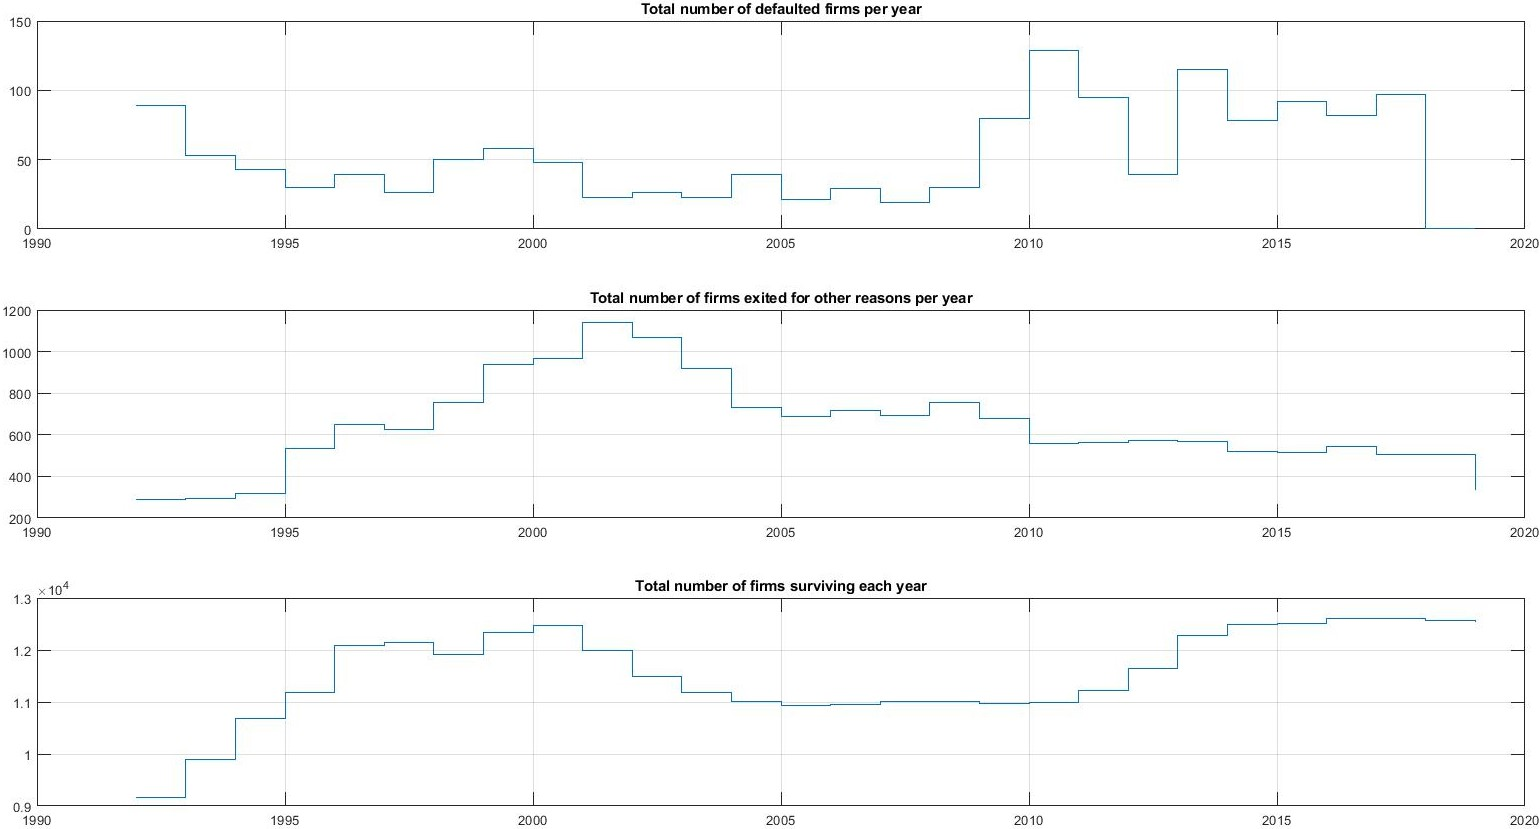
\includegraphics[width=\textwidth]{def_surv_oe_plot.jpg}
    \caption{Number of firms defaulted, exited for other reasons, surviving each year}
    \label{fig:defsurv}
\end{figure}

\begin{table}[]
    \centering
    \begin{tabular}{l l l l}
    \hline\hline
Horizon & Surviving & Defaults & Other exits \\
    \hline
0 &  2'025'094 & 499 & 10'392\\
%1 &  2'007'311 & 497 & 10'384\\
%2 &  1'989'548 & 483 & 10'173\\
3 &  1'972'063 & 514 & 10'746\\
%4 &  1'953'935 & 511 & 10'743\\
%5 &  1'935'839 & 481 & 10'503\\
6 &  1'918'061 & 499 & 10'713\\
%7 &  1'900'041 & 495 & 10'712\\
%8 &  1'882'058 & 460 & 10'433\\
%9 &  1'864'422 & 468 & 10'611\\
%10 &  1'846'587 & 463 & 10'610\\
%11 &  1'828'772 & 445 & 10'324\\
12 &  1'811'323 & 454 & 10'393\\
%13 &  1'793'797 & 453 & 10'387\\
%14 &  1'776'301 & 433 & 10'037\\
%15 &  1'759'250 & 434 & 10'073\\
%16 &  1'742'157 & 432 & 10'070\\
%17 &  1'725'084 & 416 & 9'770\\
%18 &  1'708'387 & 417 & 9'796\\
%19 &  1'691'651 & 416 & 9'793\\
%20 &  1'674'942 & 391 & 9'434\\
%21 &  1'658'690 & 392 & 9'451\\
%22 &  1'642'418 & 390 & 9'446\\
%23 &  1'626'160 & 381 & 9'183\\
24 &  1'610'242 & 382 & 9'193\\
%25 &  1'594'311 & 381 & 9'189\\
%26 &  1'578'397 & 369 & 8'863\\
%27 &  1'562'910 & 370 & 8'871\\
%28 &  1'547'409 & 370 & 8'867\\
%29 &  1'531'923 & 358 & 8'605\\
%30 &  1'516'819 & 360 & 8'606\\
%31 &  1'501'703 & 359 & 8'601\\
%32 &  1'486'610 & 342 & 8'283\\
%33 &  1'471'935 & 343 & 8'296\\
%34 &  1'457'240 & 343 & 8'295\\
35 &  1'457'240 & 343 & 8'295 \\
\hline
    \end{tabular}
    \caption{Number of firms in each category for each horizon of prediction $\tau$ which corresponds to the firm-month observations used in the likelihood for horizon $\tau$}
    \label{tab:observ}
\end{table}

\citet{leippold} used a theoretical model to show that the most powerful default predictor must incorporate both macroeconomic and accounting data. For more transparency and to allow better comparison with previous literature, I chose to work with a similar set of features similar than my benchmark model \citet{Duan2012}. Firm-specific values are common to each firm, macroeconomics variables are function of market data. The exhaustive list of variables is the following :
\begin{enumerate}
\item SP500 : trailing 1-year return on the S\&500 index. 
\item Treasury : 3-month annualized US Treasury bill rate. I use this variable as the risk-free rate $r$ in the model. 
\item DtD : the Distance-to-default is a volatility adjusted leverage measure for gauging how far is the firm from default. It was first introduced by \citet{Merton1974} model which treat firm's equity value as a call option on the underlying asset and the strike being the debt level. The DtD can be viewed as the number of standard deviations of annual asset growth by which the asset level exceeds the firm's liabilities. In this paper, the DtD is estimated using a maximum likelihood taking into account other liabilities of each firm to handle financial firm's bias. It is well-known in the literature that DtD is a significant measure to estimate default probabilities but has to be used conjointly with other variables. See the Appendix for additional information regarding the estimation procedure of DtD.
\item CASH/TA : ratio between cash and short-term investment to total assets. Both quantities are taken from the balance sheet of the company.
\item NI/TA : ratio between net income to the total assets. A loss is registered as a negative net income.
\item SIZE : logarithm of the ratio between a firm market equity value to the average market equity value of the whole S\&P500. The market equity value is computed as the stock price multiplied by the number of outstanding shares at the end of each quarter. SIZE is negative if the firm has a smaller market capitalization than the average market capitalization and positive otherwise.
\item M/B : market-to-book ratio computed using the ratio between the asset market value from the DtD maximum likelihood estimation to the total book asset value.
\end{enumerate}

To capture momentum of variables, I also compute one step rolling window differences for each firm-specific variables. These variables are called ``$\Delta$" followed by the name of variable. They are telling whether the firm has been improving or deteriorating with respect to this particular variable comparing to the last period performance. Given this model specification, the $\Delta$ is particularly interesting because if a firm shows many consecutive negative delta values, it really means the company is in danger. However, it is also important to look at the level value to compare a defaulted firm with a non-defaulted firm. The intuition tells us that prior default time, a defaulted company should have shown lower level values (for instance, DtD) than a non-defaulted firm.


\subsection{Summary statistics}
\label{sec3-2}


This section depicts the summary statistics of the dataset. Table \ref{tab:meanvar} shows a summary of the means of variables for each three categories of firm. Please note that we have to be very careful when comparing two means in this table. Comparing means needs to be done with confidence intervals and tests of significance which involves standard deviations. This table is presented to give a rough idea without performing any statistical inference. The table shows that the average defaulted firm is smaller, has a lower DtD, a smaller Market-to-book ratio, loses more money and has less cash. The prefixes $\Delta$ in front of the variables stand for the one-lag differences. Finally, Figure \ref{fig:corrmat} shows the correlation matrix for the twelve covariates.

\begin{table}[]
    \centering
    \begin{tabular}{lrrr}
    \hline \hline
                 & Surviving &   Default  & Other exits \\
    \hline
Cash/TA          &  0.1952 &  0.1896  &    0.1851 \\
NI/TA            & -0.0756 & -0.2057  &   -0.129 \\
Size             & -2.7845 & -4.6743  &   -3.621 \\
DtD              & 10.641 &  6.441  &    8.401 \\
MBratio          &  2.3774 &  1.6995  &    2.202 \\
$\Delta$ CASH/TA  & -0.0026 &  0.0023  &   -0.0074 \\
$\Delta$   NI/TA     & -0.0019 & -0.0433  &   -0.0148 \\
$\Delta$  Size      & -0.0305 & -0.5095  &   -0.0939 \\
$\Delta$   DtD       & -0.1366 & -0.7346  &    0.0295 \\
$\Delta$  MBratio   & -0.0285 &  0.0520  &    0.0801 \\
\hline
    \end{tabular}
    \caption{Mean of variables for surviving firms, defaulted firms and other exits. $\Delta$ are one period lagged differences.}
    \label{tab:meanvar}
\end{table}


\begin{figure}[]
    \centering
    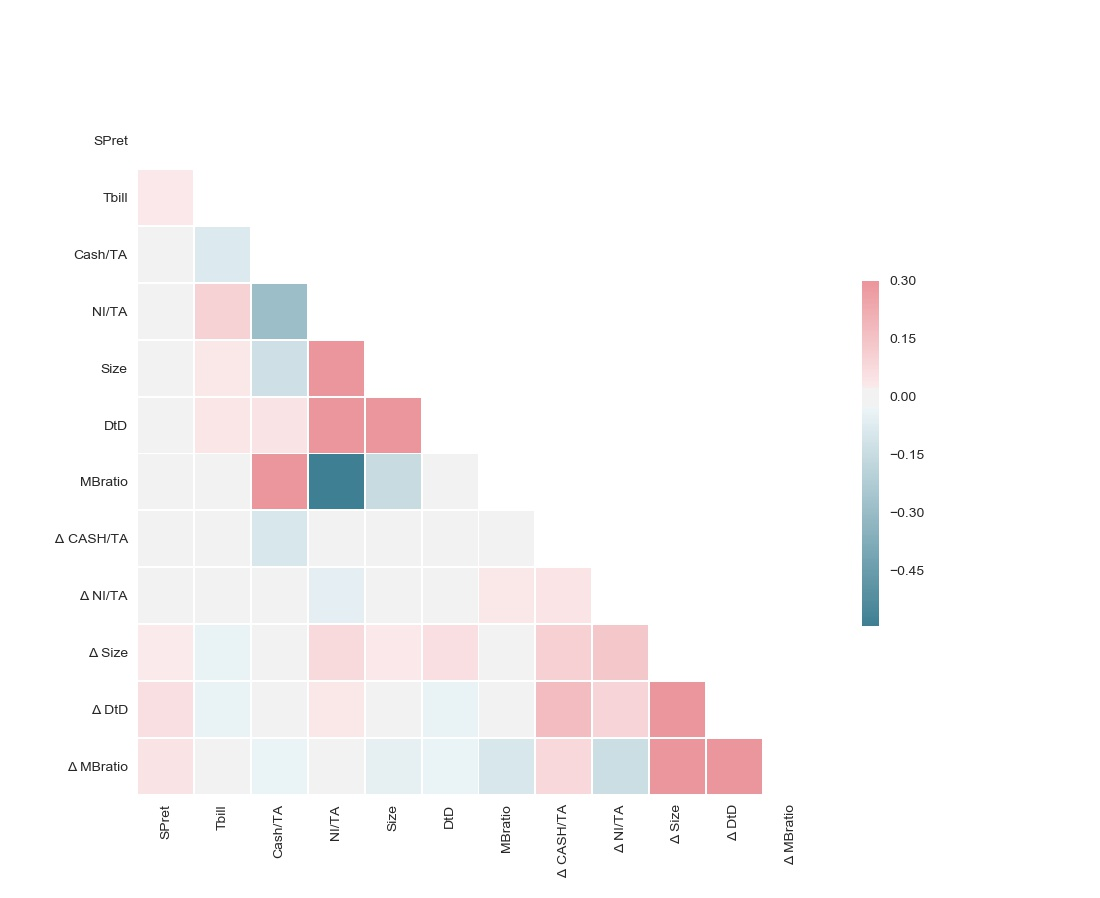
\includegraphics[scale=0.6]{corrmatrix.jpeg}
    \caption{Correlation matrix for firm-specific and macroeconomic covariates}
    \label{fig:corrmat}
\end{figure}

\section{Results}
\label{sec4}


As every neural network, we need to chose the optimal hyperparameters to achieve the highest performance. In my setup, this consists mainly of choosing the architecture of the model (i.e the number of neurons and layers). To do so, there is currently no other better method than trial and error. However, I need to be careful to not chose hyperparameters that overfit the test set. To avoid any overfitting, I perform a 5-fold cross validation for each horizon of prediction. I cut 15\% of the dataset as test set, all results that I will talk about in this chapter are out-of-sample and performed on the observations of the test set that the model has never seen before. The remaining set of observations is partitioned into smaller subsets so that in every fold of the validation a different subset is used as validation set and the rest is used as training set. Finally, to measure the discriminatory power of the models, I use the Lorenz curve (\citet{lorenz}) and I use the Gini coefficient as a scalar performance measure to aggregate across folds to get the  measure that I will use to discriminate models. \\

%Cumulative accuracy profile (CAP), also known as power curve, is often employed todetermine the performance of a rating/default prediction model. CAP is only concernedwith rankings and totally ignores the degrees of riskiness. To produce a CAP, we first lineup the obligors ranging from most risky to least risky.  Then, set a percentage and takea group of most risky obligors corresponding to this chosen percentage.  Finally, identifydefaulted obligors in this group and compute the percentage represented by these defaultedones in the population of all defaulted obligors. CAP is a plot that relates the percentageamong defaulted obligors to the percentage among the ranked obligors. In a large sample,the CAP corresponding to a perfect risk ranking model should quickly rise to one and levelat one. In contrast, a completely uninformative risk ranking model will have the CAP plotas a line with the slope equal to one.  Figure 4 presents the CAPs corresponding to thestandard and hierarchical intensity models

\begin{definition}[Lorenz curve]
The Lorenz curve of a predictor P is the two-dimensional graph
\begin{equation*}
    (\mathbb{P}\{P \leq p\},\mathbb{P}\{P\leq p | Y = 1\}),
\end{equation*}
$\forall p \in (-\infty,+\infty)$.
\end{definition}

The Lorenz curve plots on the x-axis the cumulative percentage of observations against the fraction of defaults on the y-axis.
These curves are often used in the literature for default prediction (for instance \citet{leippold}, \citet{Duan2012}) and I have seen very similar plots under two other names : power curves and cumulative accuracy profiles. They are different from ROC curves and precision-recall curves because they don't rely on thresholds to discriminate of true positives against false positives. I believe that they are particularly well-suited as performance measure in this model because of the multiperiod framework involved. The idea is that if the model is outputting a false positive for an horizon x but the true positive is horizon x+1, the model should not be ``too much" penalized. The ROC and precision-recall curves would treat this as a false positive even though the prediction was not that far from the target. The idea behind the Lorenz curve is to order default probabilities and look how they are distributed across defaulted and non-defaulted firms. We can easily see whether the model is outputting high probabilities for defaulted firms and small probabilities for surviving firms. \\
Finally, the Gini coefficient is used as my scalar summary statistic to compare models. It measures the degree of inequality of the Lorenz curve. A perfect model has a Gini coefficient close to 1 (depending on the fraction of defaults in the dataset) and a poor model has a Gini coefficient of 0 (perfect equality).

\subsection{Model choice}
\label{sec4-1}


The choice of the optimal architecture of the neural network has been made using k-fold cross-validation. The average Gini coefficient across all folds for every horizon is used as comparison tool to determine the best model architecture. If the architecture is too deep, the implicit function computed in the network to output forward intensities incorporates too many parameters and the risk of overfitting is larger, resulting in a lower accuracy measure. Similarly, if the network is not deep enough, the forward intensities are computed using a too simplistic representation and result in a low accuracy measure as well. This is usually known in the machine learning literature as the bias-variance tradeoff. Figure \ref{fig:ginicomp} shows the average Gini coefficient compute on the validation test across all folds of the cross validation for each horizon. I compare the scores obtained with different network architectures with those using the linear assumption. In this setup, one can interpret ``architecture'' as ``non-linearity degree'' as higher architecture involves more weights in the output function to be estimated. By disantangling the spaghettis, we can clearly see the bias-variance tradeoff. Increasing the depth of the networks from the simplest neural network [1] to a two layers network [2, 1] increases the Gini coefficients, in particular at mid horizons. This is probably due to the non-linearities introduced via the second layer. Next, it looks like the [3, 2] performs similarly as the [2, 1]; but we clearly see that [5, 3] dominates any other previous models. Finally, increasing the depth again to [10, 5] decreases Gini coefficient at all horizons, suggesting a severe overfitting of the forward intensities function. For next sections, I will now only show out-of-sample results of the [5, 3] architecture using the test set preliminary set on the side. \\


\begin{figure}
    \centering
    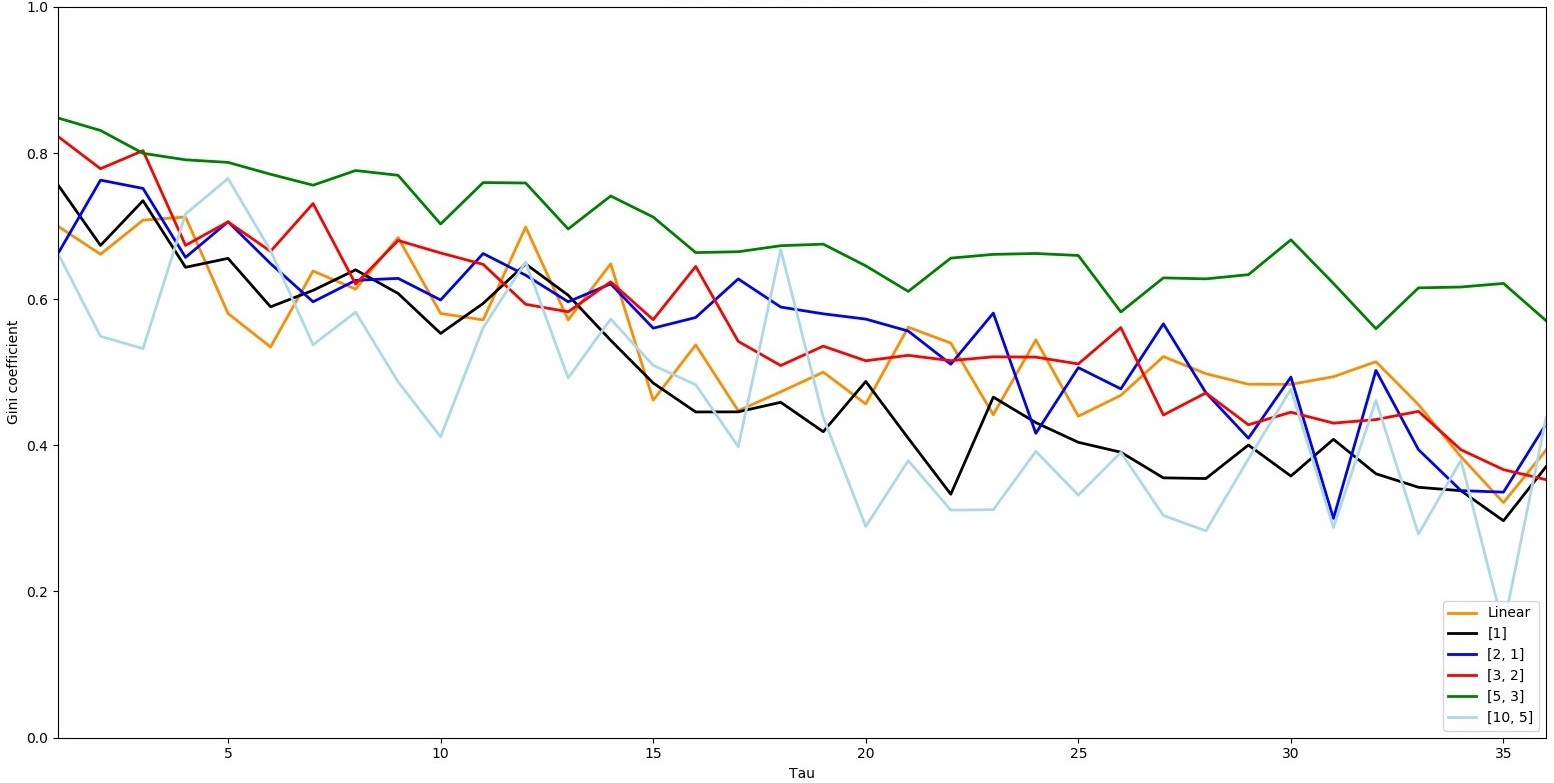
\includegraphics[width=\textwidth]{duan_vs_NN.jpeg}
    \caption{Gini coefficient : Linear vs Neural Networks}
    \label{fig:ginicomp}
\end{figure}


\subsection{Performance}
\label{sec4-2}

Figure \ref{fig:perf} shows Lorenz curves for horizon 0, 3, 6, 12, 24 and 35. Please note that all results generalize well to all others horizons. The curves are completely out-of-sample since they are computed on the test set that the model has never seen before. Table \ref{fig:ginicomp} shows Gini coefficients for both the linear assumption \citet{Duan2012} and for the [5, 3] for the same horizons. Overall, as expected the neural network clearly outperforms the linear assumption, suggesting that the linear assumption from \citet{Duan2012} can be greatly improved by adding non-linearities in the specification of the intensities. Unfortunately, it is difficult to tell which kind of non-linearities should be taken into account since neural networks are often seen as a black box. However, I will still try to answer this question by looking how the average intensity outputted by the model changes when we change a feature ceteris paribus (see section dedicated to ``sensitivities"). Another attempt at answering this question is described in the section ``computational graph'', where I deep dive into the weights of the network to understand how the output is computed.

For comparison purposes, figure \ref{fig:lor0duan} shows the Lorenz curves for both linear assumption, its replication in the neural network framework, and the [5, 3] model. The linear assumption and its replication have similar performance, suggesting again that the neural network ``NN+exp+[1]" is able to easily replicate the linear framework depicted in \citet{Duan2012}.

\begin{figure*}
        \centering
        \begin{subfigure}[b]{0.48\textwidth}
            \centering
            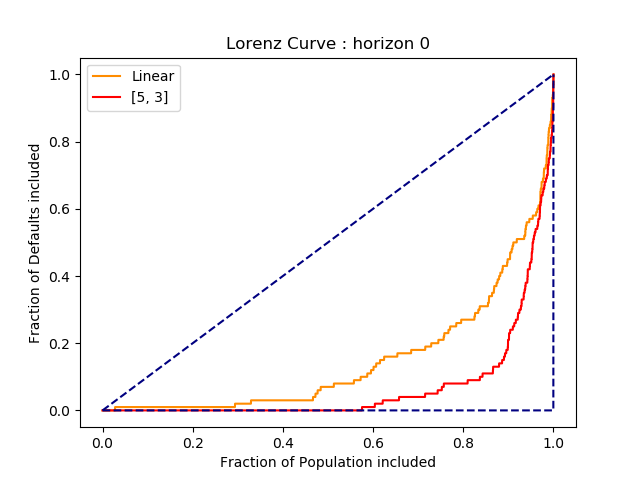
\includegraphics[width=\textwidth]{0.png}
            \caption*{Horizon 0}
        \end{subfigure}
        \quad
        \begin{subfigure}[b]{0.48\textwidth}  
            \centering 
            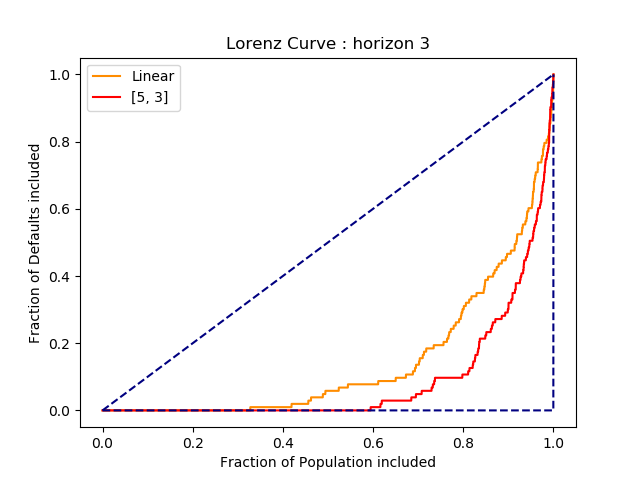
\includegraphics[width=\textwidth]{3.png}
            \caption*{Horizon 3}  
        \end{subfigure}
        \vskip\baselineskip
        \begin{subfigure}[b]{0.48\textwidth}   
            \centering 
            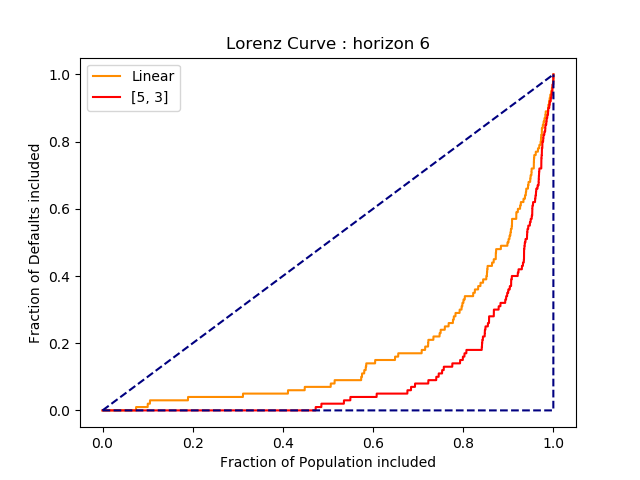
\includegraphics[width=\textwidth]{6.png}
            \caption*{Horizon 6}   
        \end{subfigure}
        \quad
        \begin{subfigure}[b]{0.48\textwidth}   
            \centering 
            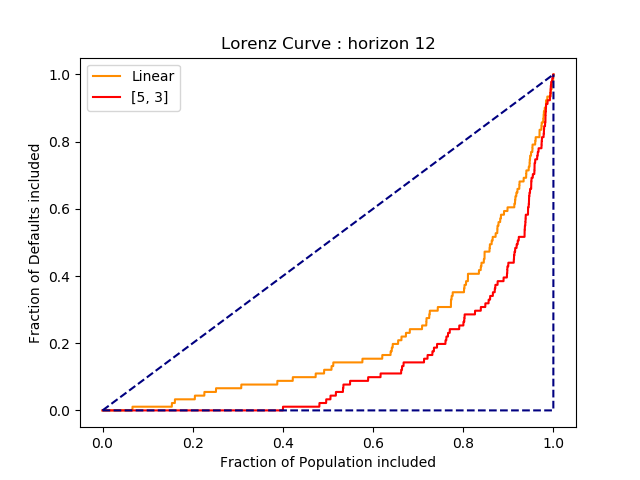
\includegraphics[width=\textwidth]{12.png}
            \caption*{Horizon 12}   
        \end{subfigure}
                \vskip\baselineskip
        \begin{subfigure}[b]{0.48\textwidth}   
            \centering 
            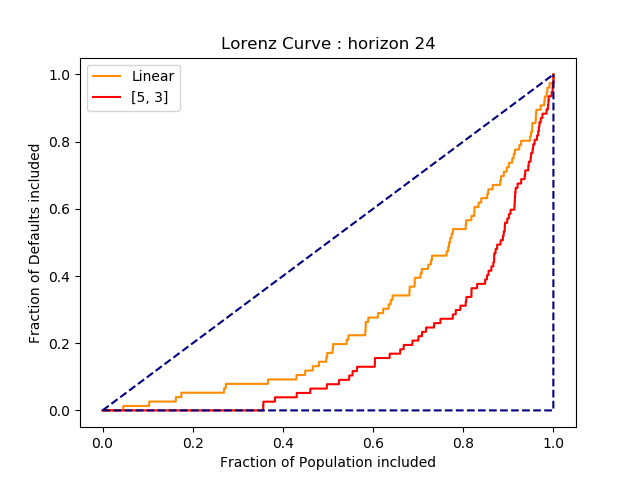
\includegraphics[width=\textwidth]{24.png}
            \caption*{Horizon 24}
        \end{subfigure}
        \quad
        \begin{subfigure}[b]{0.48\textwidth}   
            \centering 
            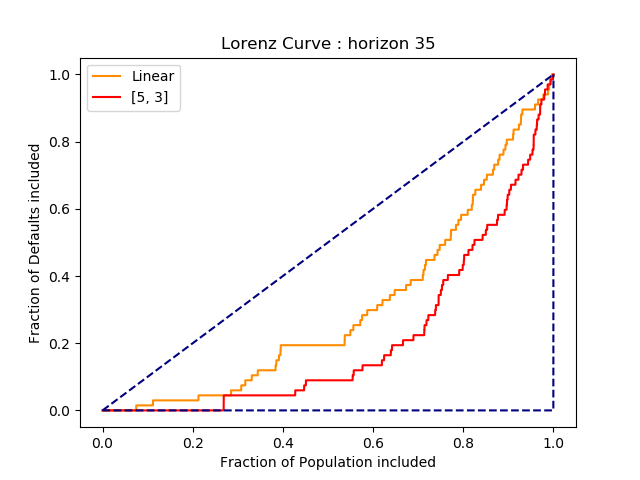
\includegraphics[width=\textwidth]{35.png}
            \caption*{Horizon 35}  
        \end{subfigure}
        \caption{Out-of-sample Lorenz Curves for each horizon. The orange line shows the performance of Duan's model and the red line shows the performance of the [5,3] neural network.} 
        \label{fig:perf}
    \end{figure*}

\begin{table}[]
    \centering
    \begin{tabular}{lll}
\hline
Horizon	&	[5, 3]	&	Linear	\\
\hline \hline
0	&	0.85	&	0.70	\\
%1	&	0.83	&	0.66	\\
%2	&	0.80	&	0.71	\\
3	&	0.79	&	0.71	\\
%4	&	0.79	&	0.58	\\
%5	&	0.77	&	0.53	\\
6	&	0.76	&	0.64	\\
%7	&	0.78	&	0.61	\\
%8	&	0.77	&	0.68	\\
%9	&	0.70	&	0.58	\\
%10	&	0.76	&	0.57	\\
%11	&	0.76	&	0.70	\\
12	&	0.70	&	0.57	\\
%13	&	0.74	&	0.65	\\
%14	&	0.71	&	0.46	\\
%15	&	0.66	&	0.54	\\
%16	&	0.66	&	0.45	\\
%17	&	0.67	&	0.47	\\
%18	&	0.68	&	0.50	\\
%19	&	0.65	&	0.46	\\
%20	&	0.61	&	0.56	\\
%21	&	0.66	&	0.54	\\
%22	&	0.66	&	0.44	\\
%23	&	0.66	&	0.54	\\
24	&	0.66	&	0.44	\\
%25	&	0.58	&	0.47	\\
%26	&	0.63	&	0.52	\\
%27	&	0.63	&	0.50	\\
%28	&	0.63	&	0.48	\\
%29	&	0.68	&	0.48	\\
%30	&	0.62	&	0.49	\\
%31	&	0.56	&	0.51	\\
%32	&	0.62	&	0.46	\\
%33	&	0.62	&	0.38	\\
%34	&	0.62	&	0.32	\\
35	&	0.57	&	0.39	\\
\hline
    \end{tabular}
    \caption{Gini coefficients}
    \label{tab:ginicoeff}
\end{table}

\begin{figure}
    \centering
    \includegraphics[width=\textwidth]{lor0duan.png}
    \caption{Comparison with the benchmark model \citet{Duan2012}. The green line shows the performance of the [1] neural network (i.e a single hidden layer with a single neuron) with an exponential activation function. The orange line shows the performance of Duan's model and the red line shows the performance of the [5,3] neural network.}
    \label{fig:lor0duan}
\end{figure}

\subsection{Computational graph}
\label{sec4-3}

Figure \ref{fig:compgraph} is a representation of a fully trained neural network for the forward default intensity $f$ at horizon 0. Negative weights are drawn as blue lines connecting neurons where orange lines show positive weights. The thicker the line, the higher the weight is in absolute value. Recall that each neuron is activated with a sigmoid function and the biases are not shown on the graph.
In the input layer, all variables seem to be used in the computation of the first layer. In the first layer however, the second neuron presents a higher weight in the network than the others. In return, the inputs connected to the second neuron of the first hidden layer all present low relative weights. Even though the computational graph gives an overview of the neural network and is useful to understand the way the output is computed, it is not trivial to see which variables have more impact on the output. In the following section, I plot sensitivities of each variable in each horizon to better understand the causality of each input.

\begin{figure}[H]
    \centering
    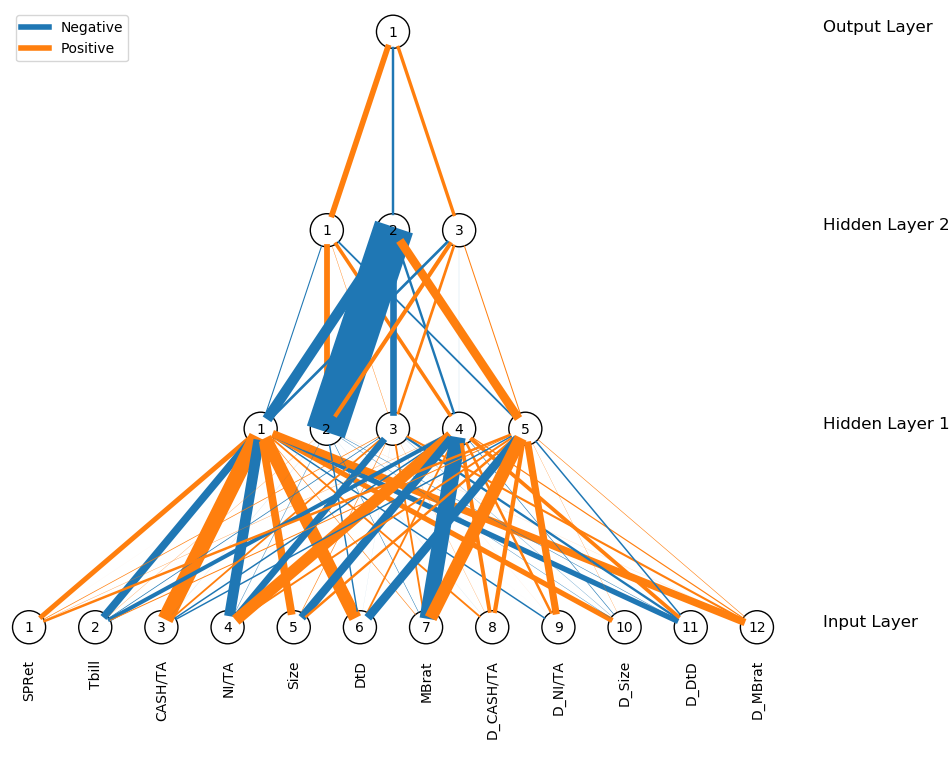
\includegraphics[width=\textwidth]{compgraphr.png}
    \caption{Trained [5, 3] Neural Network for forward default intensity at horizon 0. Negative weights are drawn as blue lines connecting neurons where orange lines show positive weights. The thicker the line, the higher the weight is in absolute value.}
    \label{fig:compgraph}
\end{figure}

\subsection{Sensitivities}
\label{sec4-4}

Neural networks are often seen as black boxes because their outputs are coming from a general function involving many parameters. It is incorporating non-linearities via the layers and the activation functions. Figure \ref{fig:sensi} is an attempt at gauging how the model reacts to a change of an input variable. It plots the average default forward intensity against a shift in the specified variable and is computed the following way:

\begin{enumerate}
    \item Compute the forward default intensity for all the observations in the test set and average the result. Then, keeping everything else equal, change the value of one feature by an absolute value and feed the ``updated" observations to the network as new input and compute the new average forward default intensity. 
    \item Repeat step 1 for all absolute values in some interval
    \item Plot the average intensity against the absolute change
    \item Repeat step 1-3 for all 11 other features.
\end{enumerate}

Keep in mind that there is a non-negativity constraint on forward intensities. A decreasing relationship means that an increase of the associated variable decreases the probability of default of the firm. A flat relationship means that the associated variable has a limited impact on the probability of default. We should expect CASH/TA, size, DtD, NI/TA, Market-to-book ratio and all their lagged differences ($\Delta$) to be decreasing. \\

First of all, most graphs show non-linear relationships, which is not surprising given the nature of the neural network specification. Moreover, all relationships are intuitive and expected. Forward intensities in both Size and $\Delta$Size are decreasing, suggesting that small firms tend to have higher likelihood of defaulting which is consistent with the ``too big to fail" paradigm. Similarly, firms with decreasing cash ($\Delta$CASH/TA $<$ 0) or low levels of CASH/TA appear to have higher probability of default. The model also predicts that firms with low NI/TA or decreasing NI/TA should have higher probability of default. Finally, forward intensities in DtD should be decreasing for all horizons to reflect that a higher distance to default makes the firm less likely to default. At horizon 0, a negative change in distance-to-default has a substantially greater effect on forward intensities than any other variables. This result is consistent with \cite{DSW}. Overall,
it appears that the most important predictors of default in this model are in short term Market-to-book ratio, DtD and CASH/TA, and in the long run NI/TA, CASH/TA, $\Delta$CASH/TA and DtD.


\begin{figure*}
\centering
        \begin{subfigure}[b]{\textwidth}   
            \centering 
            \includegraphics[width=\textwidth]{legendsensi.JPG}
            {{\small }}    
        \end{subfigure}
        \quad
        \begin{subfigure}[b]{0.475\textwidth}
            \centering
            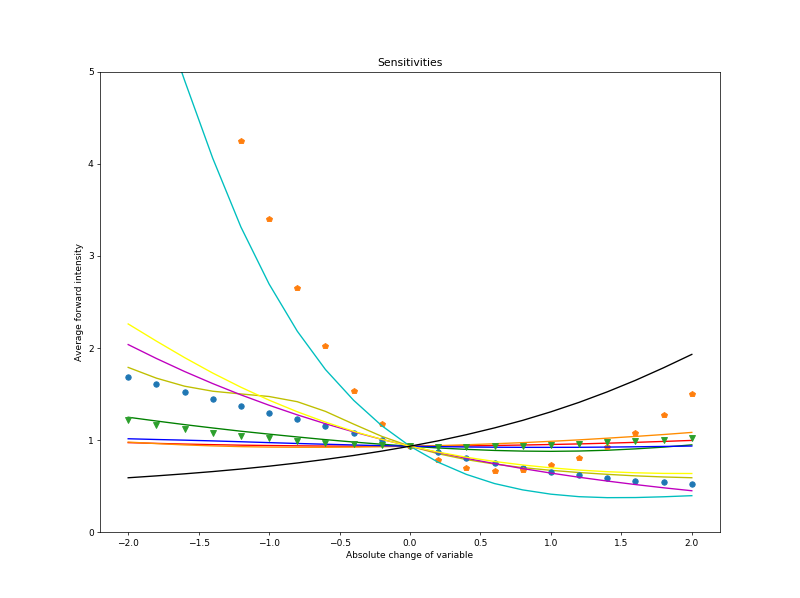
\includegraphics[width=\textwidth]{0_corr.png}
            \caption*{Horizon 0}
        \end{subfigure}
        \quad
        \begin{subfigure}[b]{0.475\textwidth}  
            \centering 
            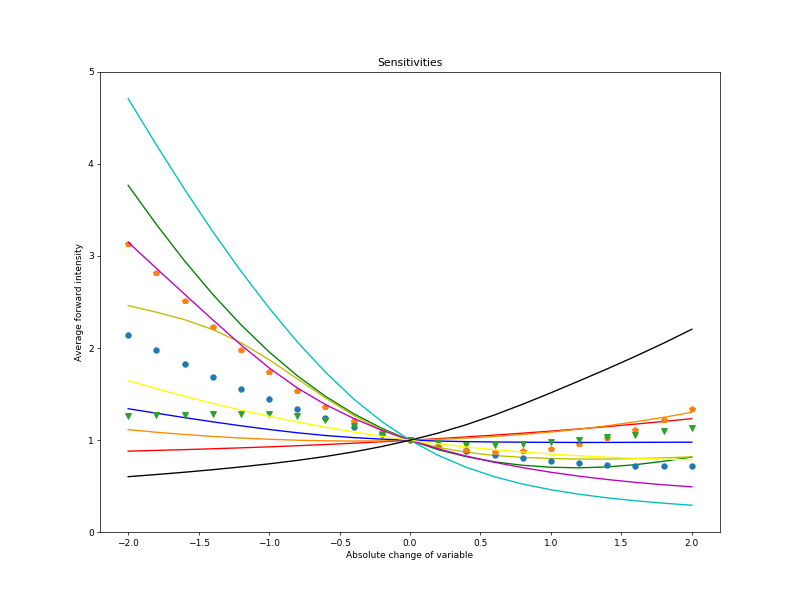
\includegraphics[width=\textwidth]{3_corr.png}
            \caption*{Horizon 3}    
        \end{subfigure}
        \vskip\baselineskip
        \begin{subfigure}[b]{0.475\textwidth}   
            \centering 
            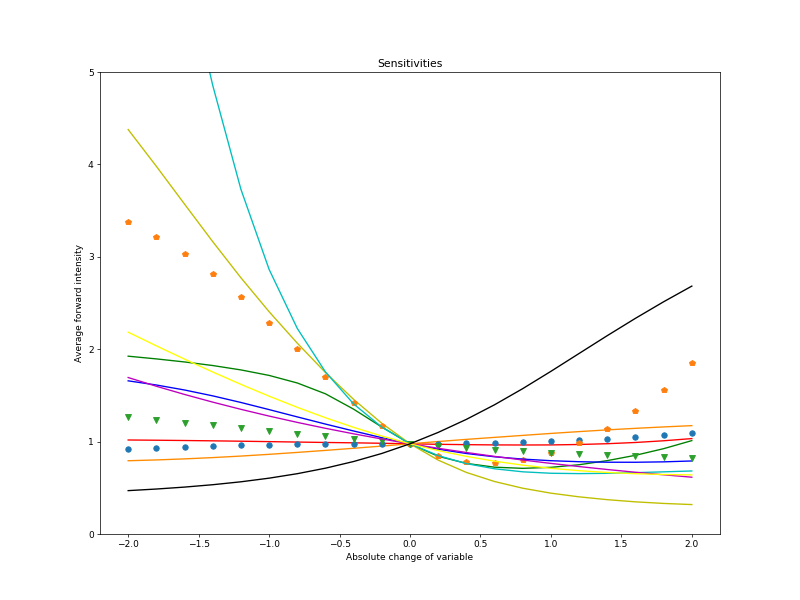
\includegraphics[width=\textwidth]{6_corr.png}
            \caption*{Horizon 6}  
            \captionsetup{position=top}
        \end{subfigure}
        \quad
        \begin{subfigure}[b]{0.475\textwidth}   
            \centering 
            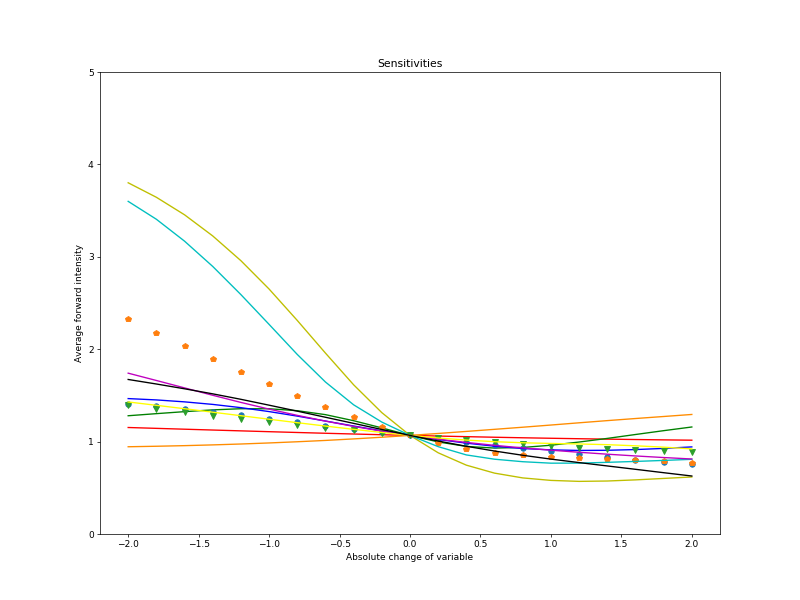
\includegraphics[width=\textwidth]{12_corr.png}
            \caption*{Horizon 12}  
            \captionsetup{position=top}
        \end{subfigure}
                \vskip\baselineskip
        \begin{subfigure}[b]{0.475\textwidth}   
            \centering 
            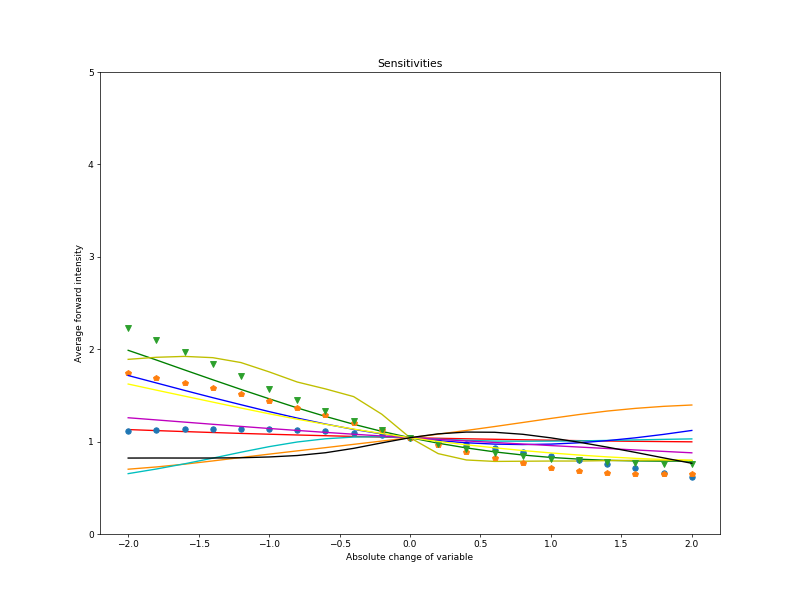
\includegraphics[width=\textwidth]{24_corr.png}
            \caption*{Horizon 24}  
        \end{subfigure}
        \quad
        \begin{subfigure}[b]{0.475\textwidth}   
            \centering 
            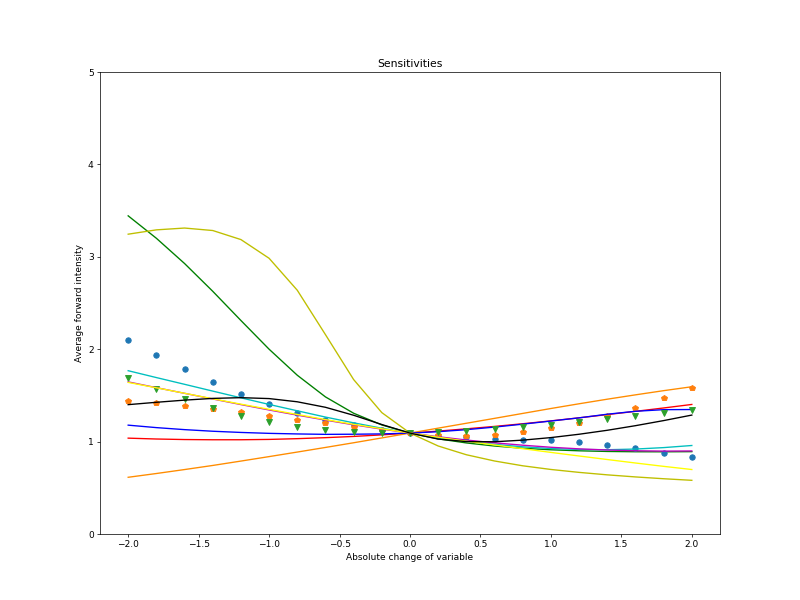
\includegraphics[width=\textwidth]{35_corr.png}
            \caption*{\small Horizon 35}
        \end{subfigure}
        \caption{Sensitivities for each horizon.} 
        \label{fig:sensi}
    \end{figure*}



\section{Conclusion}
\label{S.5}

I propose an approach to estimate default forward intensities which relies on using machine learning techniques. The key improvement over previous estimation methods is the introduction of possible highly non-linear relationships between covariates and forward intensities. Neural networks are nothing else than a very general mapping of input data to an output which is obtained by tuning weights while minimizing a given loss function. Non-linearities are introduced via the juxtaposition of layers and the activation functions. The econometric model governing the forward intensity written by \citet{Duan2012} has been adapted to this new framework to allow the use of neural networks. Neural networks are also well-suited for this paper because they allow an easy replication of the benchmark model \citet{Duan2012}. More specifically, if the network architecture is [1] (i.e : one layer and one neuron) and the activation function is chosen as being an exponential $\exp(x)$, the neural network boils down to a logit regression. The dataset used in this paper is the same as previous literature to allow easier comparison. It consists of 5 firm-specific variables computed from accounting data and 2 macroeconomic variables to control for the health of the economy. I also account for momentum of these variables by feeding the model the one lagged differences of each variable. Looking at summary statistics only, the average defaulted firm is small, has low cash, low market-to-book ratio, low Distance-to-Default and has large and negative profits. To measure the discriminatory power of the models, I follow previous literature and use Lorenz curves (also known as ``Cumulative accuracy profile" or ``Power curves"). The idea behind Lorenz curves is to order default probabilities and look how they are distributed across defaulted and non-defaulted firms. The average Gini coefficient across all folds of the cross-validation is used as comparison tool to gauge the accuracy of the model. Results show that the architecture [5, 3] (i.e 2 layers with 5 neurons in the first hidden layer and 3 neurons in the second hidden layer) seems to outperform others architecture. In this setup, one can interpret ``architecture'' as ``non-linearity degree'' as higher architecture involves more weights in the output function to be estimated. Out-of-sample Lorenz Curves and Gini coefficients show that the neural network approach outperforms the linear assumption for every horizon, suggesting the presence of non-linearities in forward default intensities. Finally, even if neural networks are known as being black boxes, one can try to see how the model reacts to a change of input variables. Most sensitivities plots show non-linear relationships, which is not surprising given the nature of the neural network specification. It appears that the most important predictors of default in this model are in the short term Market-to-book ratio, Distance-to-default and NI/TA, and in the long run NI/TA, CASH/TA, $\Delta$CASH/TA and Distance-to-default. Further works could involve more variables in the estimation. In particular, a challenging (due to lack of data) but nonetheless exciting study would be to gauge the effect of market sentiment on default intensities.



